\documentclass[10pt,letter]{article}

\usepackage{fancyhdr}
\usepackage{graphicx}
\usepackage{lastpage}
\usepackage{subfigure}
\usepackage[body={6.0in,8.0in}, left=1in, right=1in, top=1in, bottom=1in]{geometry}

\newcommand{\blankpage}{\hfill\thispagestyle{empty}\pagebreak\addtocounter{page}{-1}}

\pagestyle{fancy}
\lhead{Teaching Boxes Builder: Final Report}
\rhead{\today}

\title{Teaching Boxes Builder: \\ Final Report}
\author{Deanna Fierman  \\ \small{fierman@colorado.edu} \and
        Cory Maccarrone \\ \small{Cory.Maccarrone@colorado.edu} \and
		W. Evan Sheehan \\ \small{Wallace.Sheehan@gmail.com}}

\begin{document}
\bibliographystyle{plain}
\maketitle
\pagebreak

\pagenumbering{roman}
\tableofcontents
\cfoot{\hrule \thepage}
\pagebreak
\listoffigures
\pagebreak

\pagenumbering{arabic}
\cfoot{\hrule Page\ \thepage\ of\ \pageref{LastPage}}

\section{Problem}
Teaching boxes are digital collections of lesson plans, activities, and other
resources compiled by teachers. These compilations of materials can be utilized
by other teachers, and the lessons may be modified or added to depending on each
individual teacher's needs. Traditionally, these sets of materials are compiled
in binders or boxes, and commonly become cumbersome to use due to the amount of
material they contain.  In the Teaching Boxes Builder project, materials are
compiled and organized digitally to reduce the clumsiness of compiling large
quantities of teaching material.

Much of the digital Teaching Boxes design work is being done by DLESE (Digital
Library for Earth System Education, http://preview.dlese.org/). DLESE has a
pilot website for the digital teaching boxes\cite{bib:teachingboxes.org}.

One of the primary issues surrounding the design of digital teaching boxes is
ease of creation.  Although a teacher may have a clear lesson plan, making this
lesson and related materials available on-line has thus far been something of a
challenge.  At the present time, the teacher creates the teaching box in
Microsoft Word using a template and then sends Word document to an intermediary.
The intermediary then generates HTML from the Word document and uploads the
teaching box to the web-server. Similarly, modifying a teaching box can not be
done directly. A teacher must send the changes to someone who can propagate the
changes to the teaching box on the website.

We propose to implement a user-friendly, flexible way to allow teachers to
create teaching boxes and modify them directly. Utilizing a template provided on
the website, teachers will be able to create brand new teaching boxes that will
be immediately available to other users. It will be possible to store partially
created lessons for completion at a later time, and to modify existing teaching
boxes. The interface will need to make all the necessary steps in the creation
process clear to new users without bogging down expert users.

\section{Related Research}
We decided to primarily draw upon the readily available resources for this
project that have been written by the project sponsors.  We closely examined two
of their papers, along with looking closely at the web sites that have already
been designed for use with teaching boxes as well as other teaching lesson
websites.  In \textit{Teaching Boxes: Lessons for Digital Library Resource
Reuse} \cite{bib:khan-maull} the authors explore the components which should be
included within teaching boxes, and examine how the concept of teaching boxes
can be modified to support teachers in the most accessible way possible,
specifically as part of their current lesson-planning methods.  Several pilot
studies were run to define teaching boxes and to examine which methods of
looking at the boxes were most useful.  One of the key findings was the
necessity for extensive flexibility and adaptation for any given teacher.  The
pilot studies also found that teachers wanted detail about the lesson plans they
might be borrowing, including time required, materials, and common student
misconceptions about the subject matter.  One important note at the end of the
article is that it would be helpful to be able to connect teaching boxes to each
other.  This is an idea we have attempted to implement into our current design.

In \textit{Customizable Teaching Boxes: A Window to Digital Library Resource
Reuse} \cite{bib:khan-maull2} the authors utilized Lewis and Rieman's
task-centered design approach to examine teaching boxes in a similar fashion
that it was used in this project.  They examined the design of teaching boxes
from the perspective of lesson-planning work flow, looked at how often and in
what manner teachers modified their own lessons, and studied how they would
modify and reuse lesson plans.  They found, as we did in the current project,
that teachers rarely used prepared lessons as they were, but instead extensively
modified these lessons.  This finding formed the base of our project: designing
an easily modifiable, intuitively navigable teaching box.

\section{Approach}
We began by interviewing teachers about lesson planning -- interview questions
can be found in Appendix \ref{interview questions}, and notes from the
interviews in Appendix \ref{interview notes}. The interviews helped us gather
data regarding how teachers create lesson plans and what requirements they have
for digitizing lesson plans. The user interviews were supplemented by a survey
we sent out via e-mail -- found in Appendix \ref{survey}. This data was used to
create some low-fidelity prototypes for various aspects of the user interface.
We put these prototypes through cognitive walk-throughs and heuristic
evaluations to try and improve their design before we began any actual coding.
After evaluating the low-fidelity prototype, we created a functioning
high-fidelity prototype based on our low-fidelity mock-ups. The high-fidelity
prototype was created using XHTML, JavaScript, CSS, and AJAX. After this
prototype was complete we went back to our interviewees to have them evaluate
it. We had test users perform think-alouds on this prototype.  The feedback
gathered from the think-alouds was then used to improve the high-fidelity
prototype and create a finished project.

\section{Interviews}
We interviewed teachers from a variety of fields with varying levels of
experience, who were trying to reach different age groups, and who had different
classroom challenges, such as teaching in a bilingual classroom and teaching
deaf students.  This approach had the benefit of allowing  us to identify
consistencies in lesson planning clearly, as well as informing us of information
that was more discipline-specific.  Throughout the interviews, a handful of
common themes emerged.  One important point that arose was the need to
explicitly identify the overall question or point to the lesson, and center the
plan around that.  Oftentimes it helped teachers to have a detailed outline of
the day's lesson.  Everyone, however, mentioned how helpful it was to use
activities, laboratories, and similar sorts of things from other teachers, and
this eventually turned into one of our key design points.  Many people mentioned
the importance of adhering to state guidelines and the difficulties of knowing
which lesson plans addressed which guidelines.  Some of the teachers exchanged
lesson plans with others, and some worked together collaboratively on lesson
planning, but the primary emerging theme was that the time and energy necessary
for collaborative work was often lacking in the schools.

When a teacher borrowed another's activities, a very common practice compared to
borrowing an entire lesson, it almost always involved editing other's lesson
plan.  Not a single teacher mentioned borrowing and using a lesson plan
verbatim.  When teachers were asked about how frequently they edited and reused
their own plans, the answer was often that they did, but the ease of editing
one's own lesson plans was a crucial factor.  One problematic factor for this
particular project is that even very computer-savvy users preferred using paper
and pencil to planning lessons for the ease of carrying around and editing
on-the-spot.  Although the availability of this site as a database of lesson
plans would be a rich resource, the important question remains as to whether
teachers will actually use this in a real classroom environment.

\subsection{Individual User Profiles}
\paragraph{KK} KK taught high school science for deaf students.  She taught for
two years in Boulder county.  She now is working on an advanced degree in
education at CU-Boulder.

\paragraph{GF} GF taught middle school mathematics for twelve years, four in Trenton, NJ
and eight here in Boulder.  She did not teach classes last year but did some
tutoring at the same school she taught at, and was not teaching at all this
year. She now is working on an advanced degree in education at CU-Boulder.

\paragraph{SZ} SZ taught high school English for eight years in Illinois.  She
taught a range of classes there from introductory classes for freshmen to
senior-level Advanced Placement classes, and is currently teaching a course for
undergraduates at CU.  She now is working on her PhD in education at CU-Boulder.

\paragraph{AF} AF taught kindergarten through second grade in a Spanish-English
bilingual classroom for three years.  Currently, she's working on her PhD in
cognitive psychology at CU-Boulder.

\paragraph{JR} JR taught Spanish at Cherry Creek Middle School for three years
and high school Spanish for five years. She has taught a variety of levels from
beginning all the to senior-level classes. She now is working on an advanced
degree in Education at CU-Boulder.

\paragraph{BBS} BBS has been teaching for twelve years. She has taught Kindergarten
and first grade, and is now teaching third grade at South Elementary
School in Douglas County.

\paragraph{KW} KW taught high school social studies for thirty-five years in a second
ring Minneapolis suburb. He started teaching in a modular schedule where most of
his classes met three times a week. Later he taught in a seven-period day and finally in
a modular schedule where classes met 90 minutes a day, but for only a semester
rather than a full year.

% vim: ts=4:sw=4


\section{Abstract User Profile}
In general, our users are teachers of any grade level -- Kindergarten through
12$^{th}$ grade. They should be familiar enough with a computer to be able to
perform basic tasks: sending and receiving e-mail, browsing the Internet, or
using a word processor. The user does not necessarily need to be familiar with
the system, but a basic understanding of the teaching boxes concept is
preferred. Although our target user is a teacher, it is conceivable that anyone
involved in education might want to use this system.

\section{Design Priorities \& Issues}
From our user interviews and discussions with our sponsors we have identified
the following priorities and concerns for this project.

\subsection{Priorities}
The user interface needs to allow teachers to create digital lessons and
teaching boxes in a non-linear fashion. That is, it should not enforce an order
for the process, users should be allowed to fill in information in any order
they choose. The interface also needs to provide mechanisms for uploading files
to attach to the lesson so that teachers can include resources -- such as
worksheets -- with the lesson. Teachers should also be allowed to create links
to other lessons in the system or external web resources.

Once created, a lesson needs to be editable. As time goes on lessons are
modified and improved, so teachers need to be able to modify the digital
lessons. This also relates to the non-linearity of the interface; teachers can
begin a lesson, save it, and come back to finish it at a later date by choosing
to edit the partially complete lesson. Certain common template fields such as
materials and standards addressed should be provided by the interface. This will
help bring some structure to lessons written by different teachers and make it
easier to use and understand the lessons that a user didn't write. As well as
a number of common template fields, the interface should provide a means for
entering information not provided for by the template fields because we cannot
foresee every possible piece of information a teacher might want to include in a
lesson.

Finally, it is vital that this interface be simple and intuitive. All fields and
buttons should be clearly labeled so that their function or purpose is easily
discernible. The process of digitizing a lesson for sharing via this library
should be as painless as possible so that teachers are not dissuaded from
sharing their materials.

\subsection{Issues}
\label{sec: issues}
Activities are conceptually different from lessons. Activities are rarely
lessons in and of themselves, but frequently supplement lessons. However,
we found from our interviews that planning an activity is often quite similar to
planning a lesson; the process is often the same, some of the fields --
materials, procedure, goal, etc. -- overlap, and activities are usually
developed along with a lesson. The question that arises here is whether or not
to treat activities and lessons differently by giving them separate interfaces.
It might be confusing for users if there is no logical separation in the
interface between lesson plans and activities. But there is a risk of
duplicating much of the interface by providing separate interfaces for each.

Because creating a digital lesson can be a fairly complex task, there is a lot
of information for the user: both the information that they have entered and the
actions that they can perform on the lesson need to be visible to the user.
Thus, information visibility is a concern for this interface. We do not want to
overwhelm the user with choices and text that they've entered. But at the same
time, we do not want to make it difficult for a user to find information that
they are looking for.

Although the interface will provide a means for teachers to upload
``attachments'' to a lesson or box, there are other resources for which this is
not an adequate solution. Text books, and other hard copy resources cannot be
uploaded in this fashion. It might be possible to scan the required pages in if
there are few enough. But there needs to be some mechanism for handling
non-digital resources in lessons and boxes so that teachers are not limited to
what is already on a computer or what they can scan.

The interface provides the user with a number of common fields such as
``Methods'' and ``Materials''. These predefined fields are not always sufficient
for a lesson; a teacher might want to include information not accounted for by
these fields. It is important to allow teachers to enter whatever information
they deem important for the lesson, so a means of including this information in
a sensible fashion is important.  But we want to discourage teachers from using
these fields exclusively so that the common structure of lessons is not lost. We
do not want a teacher creating a custom field for ``Methods'' simply because
they call it ``Procedure'' and don't recognize that that is what is meant by
``Methods''.

\section{Tasks}
The following user tasks are intended to exemplify the uses of the system and
the different types of users who might find the system useful. The tasks were
derived from our user interviews.

\begin{enumerate}
\item Mrs. Anderson, a middle school English teacher for over 30 years, has a
completed lesson plan that has proven to work well over time which involves
acting out a scene in a play her class is reading. She has decided that she
would like to share this lesson with others so that they may make use of her
experiences, information, and plans.  She's familiar with paper teaching boxes
in her school, and has only begun using a computer within the last year.

\item Mr.  Multon is a second grade physical science teacher for an elementary
school. He has a lesson for an ``earthquakes'' unit, but needs to plan an
activity to accompany it.  He also has an abundance of play-doh at his disposal.

\item Ms. Frizzle just started teaching high school science this year,
and recently taught a lesson she obtained from another teacher. She found some
issues with teaching it.  For example, sometimes the chemicals that were called
for had unusual reactions, and the classroom needed to be evacuated because of
the fumes.  She would like to make notes on the lesson about her findings for
next time.

\item Mr. Johnson teaches Spanish to advanced high school students, and has done
so for five years. He is planning a lesson on food names to be taught the
following week. He has already assembled much of the information he needs, and
feels comfortable with his plan.  Two days later he gets a worksheet from a
fellow teacher on ordering at a restaurant that he thinks would add to his
lesson very nicely. He wants to incorporate it into his plan.

\item George works for the Department of Education and is developing a new
content standard to be taught at the 5$^{th}$ grade level. He wants to design a
sample lesson demonstrating how the standard could be fulfilled, and provide it
to school districts to use.

\end{enumerate}



\section{Design Approach}
Figure \ref{fig: main window} shows the main window for creating new digital
lessons. It presents the user with individual labeled text areas. These labels
will help a user identify the type of information expected in the text field.
Wherever the title might not be sufficient or ambiguous, a brief description of
the field is provided next to the title. These text fields help to add
structure to the lessons so that all lessons will be somewhat similar in format
and thus familiar and more usable.

Certain fields are optional and have a link that allows the user to remove them
from the lesson. Above the text entries is a toolbar providing the user with
formatting options and buttons with which the user can manipulate the lesson.
The area containing the text entries scrolls, but the toolbar does not. This
should make as much of the system visible to the user as possible. In many cases
it will not be feasible to display all the fields of a lesson at once, but they
are all kept on one page and should be easy to find by scrolling. The toolbar is
always available at the top, so the user never has to search the page to find
the buttons they desire. All of the buttons in the toolbar will be labeled with
text and an icon. Icons do not always clearly indicate the action performed, a
combination of descriptive text and an icon should improve a user's ability to
identify the correct button. The exception to this rule is the formatting
buttons. Formatting buttons for bold, or italic fonts, etc. are common in many
applications and will most likely be familiar to the user. In the interest of
space, these buttons only make use of icons.

There is a link at the top of this page leading to help and documentation files.
Often help buttons and menus are unhelpful; they either contain little
information, or detailed information that doesn't pertain to what most users are
interested in. This might dissuade many users from making use of a help button.
Our hope is that a link with more descriptive text about the kind of help it
provides will be less dissuasive for users in need of help.

\begin{figure}
	\centering
	\includegraphics[width=0.9\linewidth]{../../low-fi_prototype/button_mouseover}
	\caption{The basic main window for a new digital lesson.}
	\label{fig: main window}
\end{figure}

The interface for creating and modifying a teaching box (Figure \ref{fig: new box}
is even more simple than that of a new lesson. Internally, teaching boxes are
just a collection of links to lessons. There are links allowing the user to
remove one or all of the lessons contained in the box. The box contains a text
area for entering a brief description of the box that should give other users an
idea of what the box is about. The only button available to the user in the
toolbar allows the user to add another lesson to the box. Boxes are simple
enough that they can be saved automatically when the user makes a change, rather
than being explicitly saved.

\begin{figure}
	\centering
	\includegraphics[width=0.9\linewidth]{../../low-fi_prototype/teaching_box}
	\caption{The teaching box interface.}
	\label{fig: new box}
\end{figure}

The teaching boxes interface makes heavy use of dialog windows to display
additional information to the user and present them with more detailed choices.
The information in the dialog boxes is only needed by the user on rare
occasions, so most of the time it is not visible. This should help reduce
clutter on the screen and make more frequently needed information more visible.

Figure \ref{fig: dialogs} shows all of the dialogs used in this interface. When
the user elects to create a new lesson, they are presented with Figure
\ref{fig: new lesson dialog}. This dialog window allows the user to choose
additional fields to initially include in the lesson plan in addition to the
five required fields. Underneath the list of available fields the dialog
displays a brief description of the highlighted field so that if the user is
unclear about what a field is for they have more information available.

Figure \ref{fig: new field} is similar to Figure \ref{fig: new lesson dialog}. A
user is not limited to the fields with which they create a lesson, they may add
more fields later. This dialog allows the user to add fields to a lesson that
has already been created. Like the dialog in Figure \ref{fig: new lesson dialog},
this dialog provides a description of each field for the user below the list of
fields.

\begin{figure}
	\centering
	\subfigure[Dialog box shown when creating a new lesson.]{
		\label{fig: new lesson dialog}
		\includegraphics[width=0.45\linewidth]{../../low-fi_prototype/new_lesson_dialog}
	}
	\subfigure[Dialog box shown when adding more fields to a lesson.]{
		\label{fig: new field}
		\includegraphics[width=0.45\linewidth]{../../low-fi_prototype/add_field_dialog}
	}
	\subfigure[Dialog used to add a lesson to a teaching box.]{
		\label{fig: add to box}
		\includegraphics[width=0.45\linewidth]{../../low-fi_prototype/add_to_box}
	}
	\subfigure[Dialog shown when creating a new teaching box.]{
		\label{fig: new box}
		\includegraphics[width=0.45\linewidth]{../../low-fi_prototype/new_box_dialog}
	}
	\caption{Dialog windows.}
	\label{fig: dialogs}
\end{figure}

\section{Results}
\subsection{Cognitive Walk-through}
A number of problems were identified during the cognitive walk-through.  We
identified that we needed more information boxes, including ones that a teacher
could self-label since we could not identify all of the sections that a teacher
may want to use in their lesson plan.  Another problem was clarity and
consistency about what went into each of the sections in a teaching box.  The
titles of the boxes and what information needed to be included in them needed to
be specified more clearly.  There were a number of ways this issue could be
addressed, all involving giving the user more information about the section as
the box is being created and edited.  The important issue of how the information
was going to be saved was brought up, as well: how do teachers save teaching
boxes, and how frequently is saving the box necessary?  Another concern was how
teachers were going to upload materials such as worksheets to the boxes, and the
need to make this as clear as possible.  Additionally, referencing other
teaching boxes would be helpful, but could be confusing for teachers.  It would
be good to add a link near the requisite "standards this lesson meets" box to
some sort of guide to the governmental standards.

\subsection{Heuristic Evaluation}
The heuristic evaluation revealed many of the same difficulties as the cognitive
walk-through as well as a handful of new ones.  The aforementioned problem about
what to name each subsection of the lesson plan was one concern, slightly
broadened in this evaluation to consider the fact that different teachers might
call different subsections different things.  Not only do we need to be
explicitly clear, we may need to call different sections by multiple names, or
provide explicit definitions.  On the other hand, that might get very confusing.
We also realized that the user memory load of our initial design, where each
section was nested within a larger lesson plan, might be more confusing that it
needed to be.  This was caused by the lack of visibility of the subsections,
thus taxing memory load substantially.  Consistency and feedback did not appear
to be issues in our design, exits were easy to spot, and error messages seem to
only be relevant when uploading additional materials such as worksheets to the
site, a feature we have not yet designed into the interface.

\section{Final Design}
At the moment, when a teacher wants to create a lesson or box for DLESE's
library they have to type it into Microsoft Word using a template provided by
DLESE. The Word document is given to someone who administrates the DLESE
website, converted to HTML, and then added to the library. Our interface allows
users of the digital library to upload their lessons directly to the website
using a web interface instead of Microsoft Word.

For our final design we drew heavily on the DLESE website \cite{bib:preview} and
the prototype site for teaching boxes \cite{bib:teachingboxes.org}. From these
sites we gleaned the fields needed for our interface and created a look and feel
for the interface that would fit well with the existing project. We attempted to
make it as easy as possible to integrate this interface with the teaching boxes
project.

Our final design followed our low-fidelity prototype fairly closely. We used
JavaScript overlays for the dialog boxes (Figures \ref{fig: new lesson ss} and
\ref{fig: new box ss}, for example) so that the dialogs would be visible even
when the user has pop-ups disabled in their browser. We considered using a
sophisticated widget toolkit to build the interface and rejected the idea in
favor of a more simple approach. We use only standard HTML components in
conjunction with JavaScript and CSS to create the interface. This forced us to
use a simple design for the interface. It is our hope that more complex boxes
and lessons can be created by combining the simple aspects of the interface.

\begin{figure}
	\centering
	\includegraphics[width=0.45\linewidth]{figures/new_lesson}
	\caption{Dialog presented when creating a new lesson.}
	\label{fig: new lesson ss}
\end{figure}

Figure \ref{fig: blank lesson ss} shows a newly created blank lesson with some
text. Formatting options for each text area are provided beneath the text area;
formatting options are not available for all fields -- such as ``Author'' -- so
they only appear below an entry when they are available. During user testing,
many of our users did not immediately discover the formatting buttons below the
text areas. Usually after a few minutes of using the interface they realized
they were available and began using them. Beneath the name of each field a brief
description of what the field should contain is displayed.  Next to each field
name is a link that removes the field from the lesson, if the field is
removable. The user is asked to verify the removal of a field before it is
removed (Figure \ref{fig: remove prompt ss}).

\begin{figure}
	\centering
	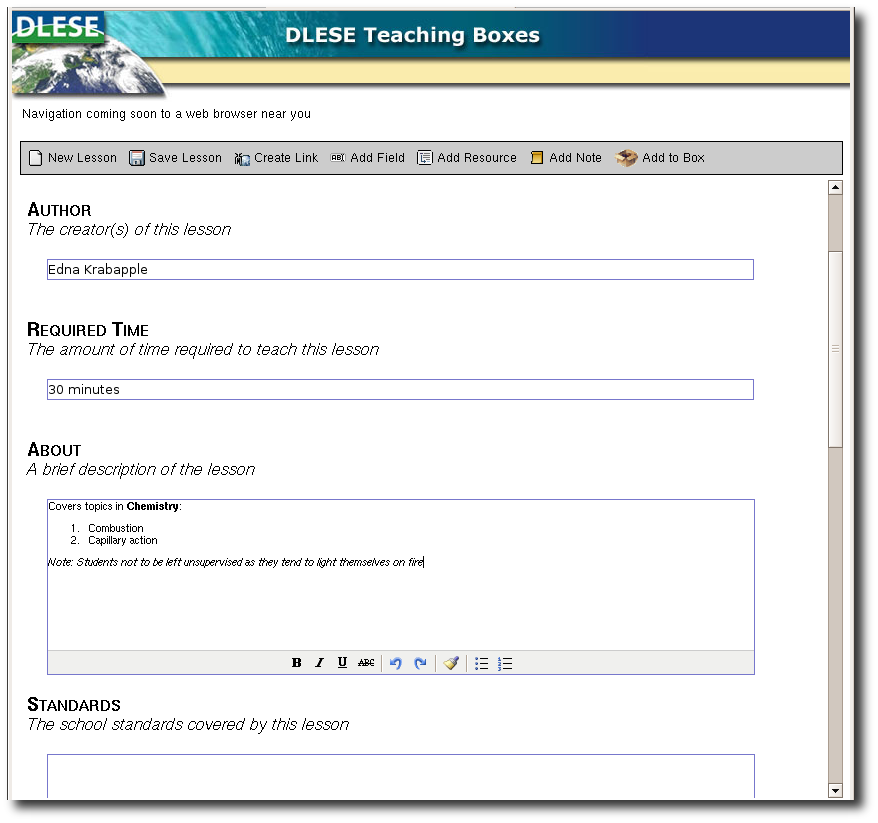
\includegraphics[width=0.9\linewidth]{figures/formatting}
	\caption{A new lesson shown with some formatted text.}
	\label{fig: blank lesson ss}
\end{figure}

\begin{figure}
	\centering
	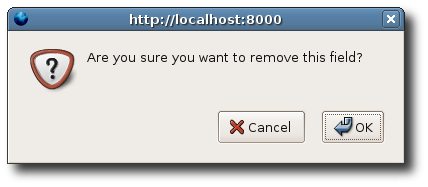
\includegraphics[width=0.45\linewidth]{figures/remove_prompt}
	\caption{Prompt presented when a user clicks ``Remove''.}
	\label{fig: remove prompt ss}
\end{figure}

The toolbar -- Figure \ref{fig: toolbar ss} -- displays text and icons for each
button. Some icons, such as the icons for ``New Lesson'' and ``Save Lesson'',
are taken from other applications that use those icons for the same action;
hopefully the icons are recognizable because of that. Other icons, such as ``Add
to Box'', are meant to directly relate to the action they perform so that their
function is easy to recognize. In case the icons are not enough to determine a
button's action, there is text next to the button that displays the button's
function. Should the text and icon not be enough, tooltips are displayed when
the cursor is placed over a button.

\begin{figure}[htb]
	\centering
	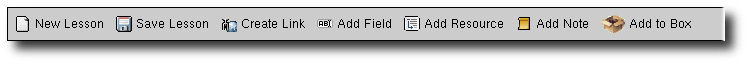
\includegraphics[width=0.9\linewidth]{figures/toolbar}
	\caption{Toolbar.}
	\label{fig: toolbar ss}
\end{figure}

\section{User Testing}
We are still setting up times to meet with users for the think-aloud, and have
two think-alouds currently scheduled.  However, the protocol is rather
straightforward.  Using the methods of Lewis and Rieman, we will ask
participants to think aloud as they perform a given task.  The user will be
asked to begin at http://lorien.navi.cx:8000/teaching\_boxes/ and create a new
lesson, one that they commonly teach.  Once they have created a lesson, their
next step will be to add a field that they "forgot" into the lesson, and to make
a note for themselves to go back and change something at a future date.  The
user will then be asked to link to a pre-existing lesson that we've uploaded
onto the server.  Once the lesson is created, they'll be asked to save it for
future use (although the actual "save" feature may not be functional).  This
walk-through should be rather short compared to the walk-throughs we did for
class exercises, primarily because of the limited number of tasks available in
this particular interface design.

After the think-aloud, users will be asked
a number of questions.  These include the following questions:

\begin{itemize}
\item What part or parts of Teaching Boxes did you find the most positive?
\item What part or parts did you find the most difficult or frustrating?
\item Looking at Teaching Boxes Builder the way it is today, do you think you'd
      use it to design your lesson plans?
      \begin{itemize}
	  \item If so, why, and if not, why not?
	  \item If so, in what ways do you think you would you use it?
	  \end{itemize}
\item Is Teaching Boxes Builder something you would use to create lessons to
	  share with other teachers?
\end{itemize}

\section{Recommendations}
During the testing phase of this project, a number of common themes emerged
regarding missing or confusing functionality. The most common request was the
ability to rearrange the fields in the interface. When the user adds new fields
to the lesson they are appended to the lesson. Many of our users expressed the
desire to move some of these fields -- e.g. ``Methods'' and ``Materials'' --
closer to the top of the lesson. It is important that the system allow users to
arrange the fields in any order they like to increase the user's comfort with
the interface. One possible solution is to add ``Rearrange Fields'' button to
the toolbar. This button could bring up a dialog with the list of fields in the
lesson that allows the user to drag-and-drop fields to different positions.

Another common request by users was for a customizable field. Often users had
one or two pieces of information they wanted to include in the lesson that was
not provided for by existing fields. Although there is a generic ``Other''
field, most users expressed the desire to rename this field to something more
specific. The primary concern with allowing users to create custom fields,
however, is that too many custom fields can destroy the consistency of lesson
formats in the library. It is important that lesson formats are consistent so
that it is not difficult for users to understand lessons they did not create.

In addition to comments from the test users, we noticed some recurring behavior
that indicated the need for some changes. A couple of the users treated the
interface as a form requesting information and allowed themselves to be guided
by the present fields. As a result, instead of adding fields for information
they wanted to include, they simply put that information in whatever fields were
already there. For example, a couple of users used the ``About'' field to define
the procedure for the lesson instead of adding a ``Methods'' field. There are a
number of possible solutions to this problem that could be investigated.

One solution is to make only ``Title'' and ``Author'' appear by default in a
lesson.  The lack of any other field should make it clear that users are free
and encouraged to add more fields to the lesson because ``Title'' and ``Author''
are not sufficient for a lesson plan by any standard. Alternatively, more
default fields could be added to the lesson. A few users expressed the desire to
have ``Methods'' be default in a lesson because all lessons have a procedure of
some kind. This solution does not stop users from allowing themselves to be
guided by the interface, but it alleviates some of the symptoms caused by this
paradigm. A third option is to leave the interface as-is and provide a tutorial
for creating lessons. A tutorial would show users how to add fields so that we
don't have to rely on them discovering it themselves. In addition to showing
them how to add fields, it suggests to the user that this is the desired
behavior for the system.

Regardless of how the above problem is addressed, we feel that a tutorial is
important. At best, it is difficult for users to divine our goals and intentions
solely from the user interface presented to them. A tutorial can clearly and
explicitly tell the user how we expect the system to be used. Then there is no
guesswork on their part regarding our expectations. The tutorial can also
explain aspects and concepts of the interface that might be difficult to
understand otherwise (such as what a teaching box is).

Finally, because this project focused primarily on the user interface, there is
some missing functionality. Lessons are not completely saved, nor is there a
storage method for lessons conducive to searching. Some issues raised in section
\ref{sec: issues} are not addressed by this project, such as the ability to cite
resources in hard copy. Obviously, in addition to the recommendations gathered
from testing, the missing functionality in this project is important.

\section{Web Analytics}
We identified two major ``business'' goals for this project: we want teachers to
contribute resources to the library, and add their lessons to the library. Both
of these goals are related to one another, but separated here so that they can
be observed individually to balance them. We would like teachers to add
resources to lessons they didn't create, as well as adding them to ones they
created.

\subsection{Control Metrics}
A simple control metric for monitoring contributed resources is simply the
number of uploads that have failed. If there are a high number of failed
uploads, there is probably something wrong with the system that is preventing
users from uploading.

For monitoring lesson/box creation we can again simply count the number of
lessons/boxes created. In addition, we can count the number of lesson/box views
per user and compare that to how many lessons/boxes they create. This will give
us an idea of how many lessons a user creates on average versus how much they
utilize the library. If this number is too low to provide a library big enough
for our taste, something needs to be done to motivate people to contribute
lessons.

\subsection{Analytic Metrics}
The number of resources uploaded compared to the number of lessons in the
library can be used to determine how much difficulty users have uploading
resources. Assuming that the reason few resources are contributed is not because
the uploads are failing, it is likely that a low number of contributed resources
is due to something in the system discouraging users from uploading resources.

Monitoring the number of creations after specific lessons have been viewed could
also be meaningful. If there are lessons that have significantly higher creation
rate after being viewed could possess some quality that motivates people to
contribute lessons. Another useful metric for this goal is how many lessons a
user viewed before creating their first lesson or box. Given enough users, this
should give some indication of how long an average user needs to utilize the
library before beginning to contribute to it.

\subsection{Moments of Truth}
There are a few scenarios in which the system can cause the user a great deal of
grief. When the user is searching the library for a resource or lesson that they
know is there, but does not appear in the search results. When a user tries to
connect a lesson to a concept that does not exist. And when a file upload fails.

\pagebreak
\appendix

\section{User Interviews}
\subsection{Questions}
\label{interview questions}
\begin{itemize}
	\item How do you create a lesson plan?

	\item Do you have a structured process, or is it different every time?

	\item How do you find resources?

	\item Do you work collaboratively?
	\begin{itemize}
		\item Do you collaborate during creation?

		\item Do you collaborate after creation?

		\item How does this process work?
	\end{itemize}

	\item How long does it take you to develop a lesson plan?

	\item What is your biggest concern when using someone else's lesson plan?

	\item What do you think you might like about using someone else's lesson
		plan?

	\item Do you know any other teachers who might like to participate?

	\item May we contact you again for later interviews or if we think of any
		further questions?
\end{itemize}

\subsection{Interview Notes}
\begingroup
\let\section\subsubsection
\label{interview notes}
\begingroup
\renewcommand{\labelenumi}{\Roman{enumi}.}
\renewcommand{\labelenumii}{\Alph{enumii}.}
\renewcommand{\labelenumiii}{\arabic{enumiii}.}
\renewcommand{\labelenumiv}{(\alpha{enumiv})}

\subsection{KK -- October 6, 2005}
\begin{enumerate}
	\item Background
		\begin{enumerate}
			\item High school science teacher
			\item Taught deaf children
			\item 2 years in Boulder County
		\end{enumerate}
	\item Creating a lesson plan
		\begin{enumerate}
			\item Work from curriculum -- identify unit goals
			\item Resources
				\begin{enumerate}
					\item Textbooks
					\item Quantity of resources increases with the newness of
						the material
				\end{enumerate}
			\item Look for activities
			\item Professional development program -- group planning
				\begin{enumerate}
					\item Discuss ``big ideas''
					\item Identify ``essential questions''
					\item Design units individually in a group setting
					\item Design assessments
					\item ``worked well''
				\end{enumerate}
		\end{enumerate}
	\item Structure
		\begin{enumerate}
			\item Begin with ``journalling question''
			\item Hands-on
		\end{enumerate}
	\item Revision process
		\begin{enumerate}
			\item Revise lessons for each class -- tailor to kids
			\item Consists largely of adding to a lesson
			\item Lab methodology
				\begin{enumerate}
					\item Changing equipment
					\item Poorly worded
				\end{enumerate}
		\end{enumerate}
	\item Sharing lessons
		\begin{enumerate}
			\item Shares labs usually, not lessons
			\item Looks for lessons on-line
			\item Always revises borrowed lessons
		\end{enumerate}
	\item What is a ``lesson plan''?
		\begin{enumerate}
			\item Objective
			\item Layout -- schedule, notes to self
			\item Questions
			\item Examples
			\item Wrap-up/conclusion -- a way to provide closure to a
				unit/lesson
		\end{enumerate}
\end{enumerate}

\subsection{GF -- October 7, 2005}
\begin{enumerate}
	\item Background -- Middle school math teacher
	\item Creating a lesson plan
		\begin{enumerate}
			\item Break year into units
			\item Break down units into lessons
			\item Determine context of lesson within unit
			\item From the context, find the lesson goal
			\item List activities
			\item Illustrations / diagrams
			\item Compile all found resources for a lesson
			\item Play around in MS Word (equation editor) -- creating
				worksheets for students, notes for self
		\end{enumerate}
	\item Collaboration
		\begin{enumerate}
			\item Casual
			\item Shared work that was done independently
			\item Modify borrowed material
			\item Write-up activity instructions when the activity is to be
				shared
		\end{enumerate}
	\item Resources
		\begin{enumerate}
			\item Text books
			\item Catalogs of teaching materials
			\item Internet (e.g. mathforum.org)
		\end{enumerate}
	\item Time scale
		\begin{enumerate}
			\item Plan year before it starts -- over the summer
			\item Plan unit before start of unit -- ideally unit preparation
				contains detailed lessons and activities for the unit
			\item Review old lessons before reuse -- sometimes rewriting,
				sometimes annotating
		\end{enumerate}
	\item What is a lesson plan?
		\begin{enumerate}
			\item Context (within unit)
			\item Goal -- various levels of specificity
			\item Sequence of activities
			\item Wrap-up / conclusion
			\item Assessment
		\end{enumerate}
\end{enumerate}

\subsection{SZ -- October 7, 2005}
\begin{enumerate}
	\item Background -- 8 years teaching high school English in Illinois
	\item Creating a lesson plan
		\begin{enumerate}
			\item Determine the course goal
			\item Create curriculum map, unit calendars
			\item Plan in detail the evening before the lesson
			\item Plans go in notebook
		\end{enumerate}
	\item Resources
		\begin{enumerate}
			\item ``Steals'' good ideas wherever she finds them
			\item Experience as a teacher and a student
			\item \textit{The English Journal}
		\end{enumerate}
	\item Structure -- Depends on class
		\begin{enumerate}
			\item Different class levels require different levels of structure
				-- Freshman intro course vs. Senior AP course
			\item AP followed a similar framework for each book
		\end{enumerate}
	\item Planning
		\begin{enumerate}
			\item Planning all the time -- solo
			\item Students help to plan discussion days
			\item Borrow and modify plans\ldots
				\begin{enumerate}
					\item From other teachers
					\item From teaching books
				\end{enumerate}
			\item Sometimes trading unit note books
		\end{enumerate}
	\item Revision
		\begin{enumerate}
			\item Much of the work goes on in her mind
			\item Keeps notes in a notebook -- details she needs to remember
			\item Re-uses maps \& calendars, never notebooks
		\end{enumerate}
	\item Notebook goes \textit{everywhere}
	\item What is a lesson plan?
		\begin{enumerate}
			\item In her head\ldots
				\begin{enumerate}
					\item Objective
					\item Material
					\item Assessment
					\item Procedure
				\end{enumerate}
			\item Notebooks
				\begin{enumerate}
					\item Contains details about the lesson or administrivia she
						needs to remember
					\item Amount of detail depends on familiarity with lesson --
						familiar lessons are largely done from memory, new
						lessons are more detailed in the notebook
				\end{enumerate}
		\end{enumerate}
\end{enumerate}

\subsection{AF -- October 12, 2005}
\begin{enumerate}
	\item Background
		\begin{enumerate}
			\item 3 years teaching grade school: 1 year each in Kindergarten,
				first, and second grade
			\item Bi-lingual classes
		\end{enumerate}

	\item Creating a lesson plan
		\begin{enumerate}
			\item Plan for the week -- it's too difficult waiting until the day
				before
			\item Start from standards, working down to curriculum and then a
				theme
			\item Backward design: kids need to learn X, how do you get to X?
			\item Resources
				\begin{enumerate}
					\item minimal resources provided by the school
					\item activities -- centers: worksheets, computers, \ldots
					\item Find resources online (about 60\%)
					\item Translate the resources into Spanish because most
						are in English -- usually the only modification
						she would make
					\item Would like to find more activities online
					\item Most online lessons didn't follow standards of
						her particular district -- would be more useful
						if they did
					\item It is hard to find resources that meet the
						needs of the students, so she would enrich
						materials found online
					\item Used other teachers as resources
					\item Went to the library for resources
					\item As a last resort invented a lesson entirely from
						scratch
				\end{enumerate}
			\item Created new lessons every year because she changed grade
				levels every year
		\end{enumerate}
	\item Collaboration
		\begin{enumerate}
			\item Mostly worked solo on planning -- small groups would form to
				share resources
			\item Willing to share her lessons/activities -- especially with
				people from whom she wanted to borrow
		\end{enumerate}
	\item Needs structure to discourage sloppiness
\end{enumerate}

\subsection{JR -- October 21, 2005}
\begin{enumerate}
	\item Background
	\begin{enumerate}
		\item Comes from a family of teachers
		\item Spanish at Cherry Creek Middle School 3 years
		\item 5 years of high school Spanish
	\end{enumerate}
	\item Lesson planning
	\begin{enumerate}
		\item Uses a big table
		\item lay out all materials -- text book, etc.
		\item Backwards design -- start from end of chapter
		\item Work from goal to requirements for achieving goal
		\item Gets easier as semester goes on
		\item Organize into categories
		\begin{enumerate}
			\item Grids of activities by category
			\item Keeps grids for future use
			\item Adds to grids when reusing
		\end{enumerate}
		\item Activities
		\begin{enumerate}
			\item Affected by level of students -- freshman vs. seniors\ldots
			\item Affected by time of day of the class -- morning vs. afternoon
			\item Geared towards individuals in class
		\end{enumerate}
	\end{enumerate}
	\item Resources
	\begin{enumerate}
		\item Coworkers
		\item Text book and related materials
		\item Internet -- resources only, not materials
	\end{enumerate}
	\item Cotaught a few lessons
	\begin{enumerate}
		\item Combining Spanish and Art
		\item Paired poor Spanish speakers with poor English speakers to help
			them learn to communicate
	\end{enumerate}
	\item Sharing lessons
	\begin{enumerate}
		\item Share rubriks
		\item Alter borrowed lessons
	\end{enumerate}
	\item Degree of teaching experience dictates how detailed a plan needs to be
	\item A lesson plan is a map of interaction with students
\end{enumerate}

\subsection{BBS -- November 27, 2005}
\begin{enumerate}
\item Creating a lesson
	\begin{enumerate}
	\item Start with standards
	\item Design a pre-test to assess where students are in relation to the goal
	\item Design a post-test to assess progress towards goal
		\begin{enumerate}
		\item Can't assume that the students got the lesson
		\item Need an assessment that determine what the students missed, not
			just that they didn't understand the lesson
		\end{enumerate}
	\item Figure out what to do with students who don't reach the goal by the
		end of the lesson and what to do with those who do
	\item Pre-assess before completing the lesson -- item If only a small group
		don't know the information, tailor the lesson to them
	\item 3 different learning styles per lesson
	\item Looks online for activities
		\begin{enumerate}
		\item Usually find overly specific lessons from college/grad students
		\item Preferes webpages run by teachers
		\item Look online before pre-test to get ideas
		\item Thinking of kids in class as she goes through the websites
		\item Download and tweak resources for the class
		\end{enumerate}
	\item Time frame
		\begin{enumerate}
		\item Depends on the amount of experience
		\item Used to take every night and all weekend as a beginning teacher
		\item Create a map for the week over the weekend as a guide for the week
		\item Plans change as soon as the students walk in
		\item Students attitude affects what they are capable of learning
		\item Especially true of Kindergarten and 1$^{st}$ grade
		\end{enumerate}
	\item Lesson structure -- mini-lesson, practice, mini-lesson, practice\ldots
	\end{enumerate}
\item Finding resources
	\begin{enumerate}
	\item Teaching books
	\item Internet
	\item Teammates
	\end{enumerate}
\item Working collaboratively
	\begin{enumerate}
		\item Meets with team to lesson plan
		\item Create a lesson as a group
		\item Process is the same as planning alone
	\end{enumerate}
\item Sharing lessons
	\begin{enumerate}
		\item Tweak borrowed lessons for the current class
		\item Other lessons act as a creative spark
		\item Concerned that it takes a lot of time to write down a lesson for
			sharing
	\end{enumerate}
\item What is a lesson plan
	\begin{enumerate}
	\item Goal (standards) -- what students need to know
	\item How to achieve goal
	\item How to assess progress towards goal and what to do with those who
		achieve the goal and those who don't
	\item Accounting for high-level, low-level, and ESL students
	\item Good teaching takes into account not only the skills to teach, but
		application of the skills learned -- learning how to think
	\item Students have to participate in the planning/learning
	\end{enumerate}
\end{enumerate}

\endgroup
% vim: ts=4:sw=4

\endgroup

\section{Survey}
The following survey was e-mailed to teachers that we couldn't interview in
person due to geographic or temporal constraints as a means of supplementing
data gathered from our interviews.

\subsection{Questions}
\begin{itemize}
\item How do you create lesson plans?  Is it a structured process, or different
      every time?
\item How do you revise lesson plans, and how frequently?
\item How long does it usually take you to create a lesson plan?
\item What goes into your lesson plans?  What are you explicit about, and what
      do you leave to memory?
\item Where do you get ideas for lesson plans?
\item How do you integrate state guidelines into your planning?
\item How do you find resources for lesson plans?
\item Do you work collaboratively with other teachers?  If you do, at what point
      in the process do you collaborate?  How does that process work?
\item What's your biggest concern about using someone else's lesson plan?
\item What do you think you might like about using someone else's lesson plan?
\item What does the term "lesson plan" mean for you?
\item Do you have any other things about lesson planning that you'd like to tell
      us?  We'd appreciate hearing whatever comments you'd like to share.
\end{itemize}

\subsection{Responses}
Verbatim responses to the survey:

\subsubsection{KW -- October 24, 2005}
Okay, Deanna,

I'm retired. So I actually have time to respond to your questions. When I was in
the throes of teaching, I probably wouldn't have time to respond -- or do to
many lesson plans.

Taught high school social studies for 35 years in a second ring Minneapolis
suburb. I started teaching in a modular schedule where most of my classes met 3
times a week. Later I taught in a 7-period day and finally in a modular schedule
where classes met 90 minutes a day, but for only a semester rather than a full
year.

For me, lesson plans came out of outlines for units that were usually 4-9 weeks
long. Once the topics for the unit were in some kind of order for learning, I'd
begin dreaming up ways to teach the topics.  The only time I worked without at
least one partner was when I taught AP classes. Unit and lesson planning were
group projects.  Lessons usually developed from objectives and available
materials; rarely from wonderfully creative inventions. For me it was never
structured -- I was always starting over. Revise? Often I didn't remember from
one year to the next what I'd done. (I had one young man who three times took a
course I taught. He frequently complained, "That's not what we did last year.")
Some things worked so well, I would remember them if the same topic became part
of the unit outline and I'd try to recreate them.

Lesson plans take from 5 minutes to 5 weeks to create. At a minimum, a lesson
plan is a scrap of paper in my pocket with a list of topics or events on it. (By
the time I got to class, I usually didn't have to look at it.) At most it was a
detailed script of what I wanted to say and do along with expected responses
(that was often the case when I introduced new topics in philosophy). Once I had
a clear idea of what the purpose of a lesson or a class was, coming up with a
lesson plan was a matter of deciding what processes would best move toward that
purpose.

Ideas come from other people, books of lesson plans (see The Center for Learning
-- http://www.centerforlearning.org/), experience, inspiration, improvisation,
and in-class interactions (some lesson plans are created in class -- "teachable
moments" don't you know).

State guidelines were considered when planning units of study, not lesson plans.

Resources are a problem. The Web helped a lot when it came along. Before that I
collected lots of original sources or collections of original sources, newspaper
and magazine articles. And when I had time (think July and August), I haunted
college and university libraries looking for documents, maps, and readings.
During most of my teaching career, I did not use textbooks -- except for the AP
courses, so I was always scrounging for material.

Collaboration can work in many ways. I think it depends upon the people involved
and the task at hand. For me, it was best when collaboration extended from
beginning to end. I knew we were successfully working together when we could
agree to give the same test at the end of a unit. Collaboration requires
agreement on goals, objectives, and main topics. It does not require agreement
on teaching methods. I am convinced that teachers teach best when they teach in
ways that make sense to them. They are better able to help students learn then.

When I use someone else's lesson plan, I'm concerned that I may get into the
lesson and realize I've missed a crucial step in learning the objective. Then I
won't know how to teach it. I loved using others' lesson plans since I didn't
have to be the creative force for a bit.

BTW, I did a "unit" of 40 lesson plans for The Center for Learning (AP
Comparative Government and Politics; to be published in November) and I learned
a great deal about preparing lessons for people I don't work with. TCL has a
very structured format for creating lesson plans for their "units." You might
want to ask them. (Or ask me and I'll try to dig up the format information they
coached me through when I was working on lessons last spring.)

\pagebreak
\bibliography{resources}

\end{document}

% vim: ts=4:sw=4
